%%%%%%%%%%%%%%%%%%%%%%%%%%%%%%%%%%%%%%%%%%%%%%%%%%%%%%%%%%%%%%%%%%%%%%%%%%%%%%%
%                                                                             %
% Copyright (C) 2007,2012 Sebastien Morin                                     %
% Copyright (C) 2012-2014 Edward d'Auvergne                                   %
%                                                                             %
% This file is part of the program relax (http://www.nmr-relax.com).          %
%                                                                             %
% This program is free software: you can redistribute it and/or modify        %
% it under the terms of the GNU General Public License as published by        %
% the Free Software Foundation, either version 3 of the License, or           %
% (at your option) any later version.                                         %
%                                                                             %
% This program is distributed in the hope that it will be useful,             %
% but WITHOUT ANY WARRANTY; without even the implied warranty of              %
% MERCHANTABILITY or FITNESS FOR A PARTICULAR PURPOSE.  See the               %
% GNU General Public License for more details.                                %
%                                                                             %
% You should have received a copy of the GNU General Public License           %
% along with this program.  If not, see <http://www.gnu.org/licenses/>.       %
%                                                                             %
%%%%%%%%%%%%%%%%%%%%%%%%%%%%%%%%%%%%%%%%%%%%%%%%%%%%%%%%%%%%%%%%%%%%%%%%%%%%%%%


% Consistency testing.
%%%%%%%%%%%%%%%%%%%%%%

\chapter{Consistency testing}
\index{consistency testing|textbf}


% Introduction.
%%%%%%%%%%%%%%%

\section{Introduction to the consistency testing of relaxation data}

In spin relaxation, datasets are often recorded at different magnetic fields.
This is especially important when $\Rtwo$ values are to be used since $\mu$s-ms motions contribute to $\Rtwo$.
This contribution being scaled quadratically with the strength of the magnetic field, recording at multiple magnetic fields helps extract it.
Also, acquiring data at multiple magnetic fields allows over-determination of the mathematical problems, e.g.\ in the model-free approach.

Recording at multiple magnetic fields is a good practice.
However, it can cause artifacts if those different datasets are inconsistent.
Inconsistencies can originate from, inter alia, the sample or the acquisition.
Sample variations can be linked to changes in temperature, concentration, pH, etc.
Water suppression is the main cause of acquisition variations as it affect relaxation parameters (especially NOE) of exposed and exchangeable moieties (e.g.\ the NH moiety).

It is thus a good idea to assess consistency of datasets acquired at different magnetic fields.
For this purpose, three tests are implemented in relax.
They are all based on the same principle -- calculate a field independent value and compare it from one field to another.

The three tests are:
\begin{description}
  \item[$J(0)$]  The spectral density at the zero frequency calculated using the reduced spectral density approach.
  \item[$F_\eta$]  A consistency function proposed by \citet{Fushman98}.
  \item[$F_{R_2}$]  A consistency function proposed by \citet{Fushman98}.
\end{description}

These three tests are very similar (all probing consistency of $R_2$ data and all suffering from the same limitations) and any of them can be used for consistency testing.
In the example below, the $J(0)$ values are used for consistency testing.

Different methods exist to compare tests values calculated from one field to another.
These include correlation plots and histograms, and calculation of correlation, skewness and kurtosis coefficients.
The details of how to interpret such analyses are avaliable at the end of this chapter in Section~\ref{sec: Visualisation and data output}.

For more details on the tests and their implementation within relax, see:
\begin{itemize}
  \item \bibentry{MorinGagne09a}
\end{itemize}

Or for the origin of the tests themselves:
\begin{itemize}
  \item \bibentry{Fushman99}
\end{itemize}

In addition, see the following review which includes a discussion on how to evaluate the reliability of recorded relaxation data:
\begin{itemize}
  \item \bibentry{Morin11}
\end{itemize}



% Script UI.
%%%%%%%%%%%%

\section{Consistency testing in the prompt/script UI mode}

The consistency testing analysis is only available via the prompt/script UI modes -- no GUI auto-analysis has yet been built by a relax power-user.


% The sample script.
%~~~~~~~~~~~~~~~~~~~

\subsection{Consistency testing script mode -- the sample script} \label{sect: consistency tests - sample script}

The following script can be found in the \directory{sample\osus{}scripts} directory.

\begin{lstlisting}
""" Script for consistency testing.

Severe artifacts can be introduced if model-free analysis is performed from inconsistent multiple magnetic field datasets. The use of simple tests as validation tools for the consistency assessment can help avoid such problems in order to extract more reliable information from spin relaxation experiments. In particular, these tests are useful for detecting inconsistencies arising from R2 data. Since such inconsistencies can yield artificial Rex parameters within model-free analysis, these tests should be use routinely prior to any analysis such as model-free calculations.

This script will allow one to calculate values for the three consistency tests J(0), F_eta and F_R2. Once this is done, qualitative analysis can be performed by comparing values obtained at different magnetic fields. Correlation plots and histograms are useful tools for such comparison, such as presented in Morin & Gagne (2009a) J. Biomol. NMR, 45: 361-372.


References
==========

The description of the consistency testing approach:

    Morin & Gagne (2009a) Simple tests for the validation of multiple field spin relaxation data. J. Biomol. NMR, 45: 361-372. U{http://dx.doi.org/10.1007/s10858-009-9381-4}

The origins of the equations used in the approach:

    J(0):
        Farrow et al. (1995) Spectral density function mapping using 15N relaxation data exclusively. J. Biomol. NMR, 6: 153-162. U{http://dx.doi.org/10.1007/BF00211779}

    F_eta:
        Fushman et al. (1998) Direct measurement of 15N chemical shift anisotropy in solution. J. Am. Chem. Soc., 120: 10947-10952. U{http://dx.doi.org/10.1021/ja981686m}

    F_R2:
        Fushman et al. (1998) Direct measurement of 15N chemical shift anisotropy in solution. J. Am. Chem. Soc., 120: 10947-10952. U{http://dx.doi.org/10.1021/ja981686m}

A study where consistency tests were used:

    Morin & Gagne (2009) NMR dynamics of PSE-4 beta-lactamase: An interplay of ps-ns order and us-ms motions in the active site. Biophys. J., 96: 4681-4691. U{http://dx.doi.org/10.1016/j.bpj.2009.02.068}
"""

# Create the data pipe.
name = 'consistency'
pipe.create(name, 'ct')

# Set up the 15N spins.
sequence.read('noe.600.out', res_num_col=1)
spin.name(name='N')
spin.element(element='N')
spin.isotope(isotope='15N', spin_id='@N')

# Load the relaxation data.
relax_data.read(ri_id='R1_600',  ri_type='R1',  frq=600.0*1e6, file='r1.600.out', res_num_col=1, data_col=3, error_col=4)
relax_data.read(ri_id='R2_600',  ri_type='R2',  frq=600.0*1e6, file='r2.600.out', res_num_col=1, data_col=3, error_col=4)
relax_data.read(ri_id='NOE_600', ri_type='NOE', frq=600.0*1e6, file='noe.600.out', res_num_col=1, data_col=3, error_col=4)

# Generate the 1H spins for the magnetic dipole-dipole interaction.
sequence.attach_protons()

# Define the magnetic dipole-dipole relaxation interaction.
interatom.define(spin_id1='@N', spin_id2='@H', direct_bond=True)
interatom.set_dist(spin_id1='@N', spin_id2='@H', ave_dist=1.02 * 1e-10)

# Define the chemical shift relaxation interaction.
value.set(val=-172 * 1e-6, param='csa')

# Set the angle between the 15N-1H vector and the principal axis of the 15N chemical shift tensor
value.set(val=15.7, param='orientation')

# Set the approximate correlation time.
value.set(val=13 * 1e-9, param='tc')

# Set the frequency.
consistency_tests.set_frq(frq=600.0 * 1e6)

# Consistency tests.
minimise.calculate()

# Monte Carlo simulations.
monte_carlo.setup(number=500)
monte_carlo.create_data()
minimise.calculate()
monte_carlo.error_analysis()

# Create grace files.
grace.write(y_data_type='j0', file='j0.agr', force=True)
grace.write(y_data_type='f_eta', file='f_eta.agr', force=True)
grace.write(y_data_type='f_r2', file='f_r2.agr', force=True)

# View the grace files.
grace.view(file='j0.agr')
grace.view(file='f_eta.agr')
grace.view(file='f_r2.agr')

# Finish.
results.write(file='results', force=True)
state.save('save', force=True)
\end{lstlisting}

This is similar in spirit to the reduced spectral density mapping sample script (Chapter~\ref{ch: J(w) mapping} on page~\pageref{ch: J(w) mapping}).


% Data pipe and spin system setup.
%%%%%%%%%%%%%%%%%%%%%%%%%%%%%%%%%%

\section{Consistency testing script mode -- data pipe and spin system setup}

The steps for setting up relax and the data model concept are described in full detail in Chapter~\ref{ch: data model}.
The first step, as for all analyses in relax, is to create a data pipe for storing all the data:

\begin{lstlisting}[firstnumber=31]
# Create the data pipe.
name = 'consistency'
pipe.create(name, 'ct')
\end{lstlisting}

Then, in this example, the $^{15}$N spins are created from one of the NOE relaxation data files (Chapter~\ref{ch: NOE}):

\begin{lstlisting}[firstnumber=35]
# Set up the 15N spins.
sequence.read('noe.600.out', res_num_col=1)
spin.name(name='N')
spin.element(element='N')
spin.isotope(isotope='15N', spin_id='@N')
\end{lstlisting}

Skipping the relaxation data loading, the next part of the analysis is to create protons attached to the nitrogens for the magnetic dipole-dipole relaxation interaction:

\begin{lstlisting}[firstnumber=46]
# Generate the 1H spins for the magnetic dipole-dipole interaction.
sequence.attach_protons()
\end{lstlisting}

This is needed to define the magnetic dipole-dipole interaction which governs relaxation.



% Relaxation data loading.
%%%%%%%%%%%%%%%%%%%%%%%%%%

\section{Consistency testing script mode -- relaxation data loading}

The loading of relaxation data is straight forward.
This is performed prior to the creation of the proton spins so that the data is loaded only into the $^{15}$N spin containers and not both spins for each spin system.
Note that if the relaxation data files contain spin information, then this order is not important.
For this analysis, only data for a single field strength can be loaded:

\begin{lstlisting}[firstnumber=41]
# Load the relaxation data.
relax_data.read(ri_id='R1_600',  ri_type='R1',  frq=600.0*1e6, file='r1.600.out', res_num_col=1, data_col=3, error_col=4)
relax_data.read(ri_id='R2_600',  ri_type='R2',  frq=600.0*1e6, file='r2.600.out', res_num_col=1, data_col=3, error_col=4)
relax_data.read(ri_id='NOE_600', ri_type='NOE', frq=600.0*1e6, file='noe.600.out', res_num_col=1, data_col=3, error_col=4)
\end{lstlisting}

The frequency of the data must also be explicitly specified:

\begin{lstlisting}[firstnumber=62]
# Set the frequency.
consistency_tests.set_frq(frq=600.0 * 1e6)
\end{lstlisting}



% Relaxation interactions.
%%%%%%%%%%%%%%%%%%%%%%%%%%

\section{Consistency testing script mode -- relaxation interactions}

Prior to calculating the $J(0)$, $F_\eta$, and $F_{R_2}$ values, the physical interactions which govern relaxation of the spins must be defined.
For the magnetic dipole-dipole relaxation interaction, the user functions are:

\begin{lstlisting}[firstnumber=49]
# Define the magnetic dipole-dipole relaxation interaction.
interatom.define(spin_id1='@N', spin_id2='@H', direct_bond=True)
interatom.set_dist(spin_id1='@N', spin_id2='@H', ave_dist=1.02 * 1e-10)
\end{lstlisting}

For the chemical shift relaxation interaction, the user function call is:

\begin{lstlisting}[firstnumber=53]
# Define the chemical shift relaxation interaction.
value.set(val=-172 * 1e-6, param='csa')
\end{lstlisting}

For the angle in degrees between the $^{15}$N-$^1$H vector and the principal axis of the $^{15}$N chemical shift tensor, the user function call is:

\begin{lstlisting}[firstnumber=56]
# Set the angle between the 15N-1H vector and the principal axis of the 15N chemical shift tensor
value.set(val=15.7, param='orientation')
\end{lstlisting}


% Calculation and error propagation.
%%%%%%%%%%%%%%%%%%%%%%%%%%%%%%%%%%%%

\section{Consistency testing script mode -- calculation and error propagation}

Optimisation for this analysis is not needed as this is a direct calculation.
Therefore the $J(0)$, $F_\eta$, and $F_{R_2}$ values are simply calculated with the call:

\begin{lstlisting}[firstnumber=65]
# Consistency tests.
minimise.calculate()
\end{lstlisting}

The propagation of errors is more complicated.
The Monte Carlo simulation framework of relax can be used to propagate the relaxation data errors to the spectral density errors.
As this is a direct calculation, this collapses into the standard bootstrapping method.
The normal Monte Carlo user functions can be called:

\begin{lstlisting}[firstnumber=68]
# Monte Carlo simulations.
monte_carlo.setup(number=500)
monte_carlo.create_data()
minimise.calculate()
monte_carlo.error_analysis()
\end{lstlisting}

In this case, the \uf{monte\ufus{}carlo\ufsep{}initial\ufus{}values} user function call is not required.


% Visualisation and data output.
%%%%%%%%%%%%%%%%%%%%%%%%%%%%%%%%

\section{Consistency testing script mode -- visualisation and data output}
\label{sec: Visualisation and data output}

The rest of the script is used to output the results to 2D Grace files for visualisation (the \uf{grace\ufsep{}view} user function calls will launch Grace with the created files), and the output of the values into plain text files.

However, simply visualizing the calculated $J(0)$, $F_\eta$, and $F_{R_2}$ values this way does not allow proper consistency testing.
Indeed, for assessing the consistency of relaxation data using these tests, different methods exist to compare values calculated from one field to another.
These include correlation plots and histograms, and calculation of correlation, skewness and kurtosis coefficients.

To complete the consistency testing analysis, the following steps are needed:
\begin{itemize}
  \item Extract the $J(0)$ values at multiple magnetic fields.
  \item Join together the data from a pair of magnetic fields either by pasting them as two columns of one file (approach A), or by dividing values from a first magnetic field by values from a second magnetic field (approach B).
  \item Make either a correlation plot (approach A), or an histogram of the ratios (approach B).
  \item See if the correlation plot is centered around a perfect correlation or skewed away (approach A), or if the values are centered around 1 in the histogram (approach B).
    If yes, data from multiple magnetic fields is consistent from one magnetic field to another.
    If no, data is inconsistent.
    In the case where inconsistency arises, if data from more than two magnetic fields is available, more than one pair of data can be checked and the inconsistent magnetic field data can be identified.
\end{itemize}

\begin{figure*}[h]
  \centerline{
    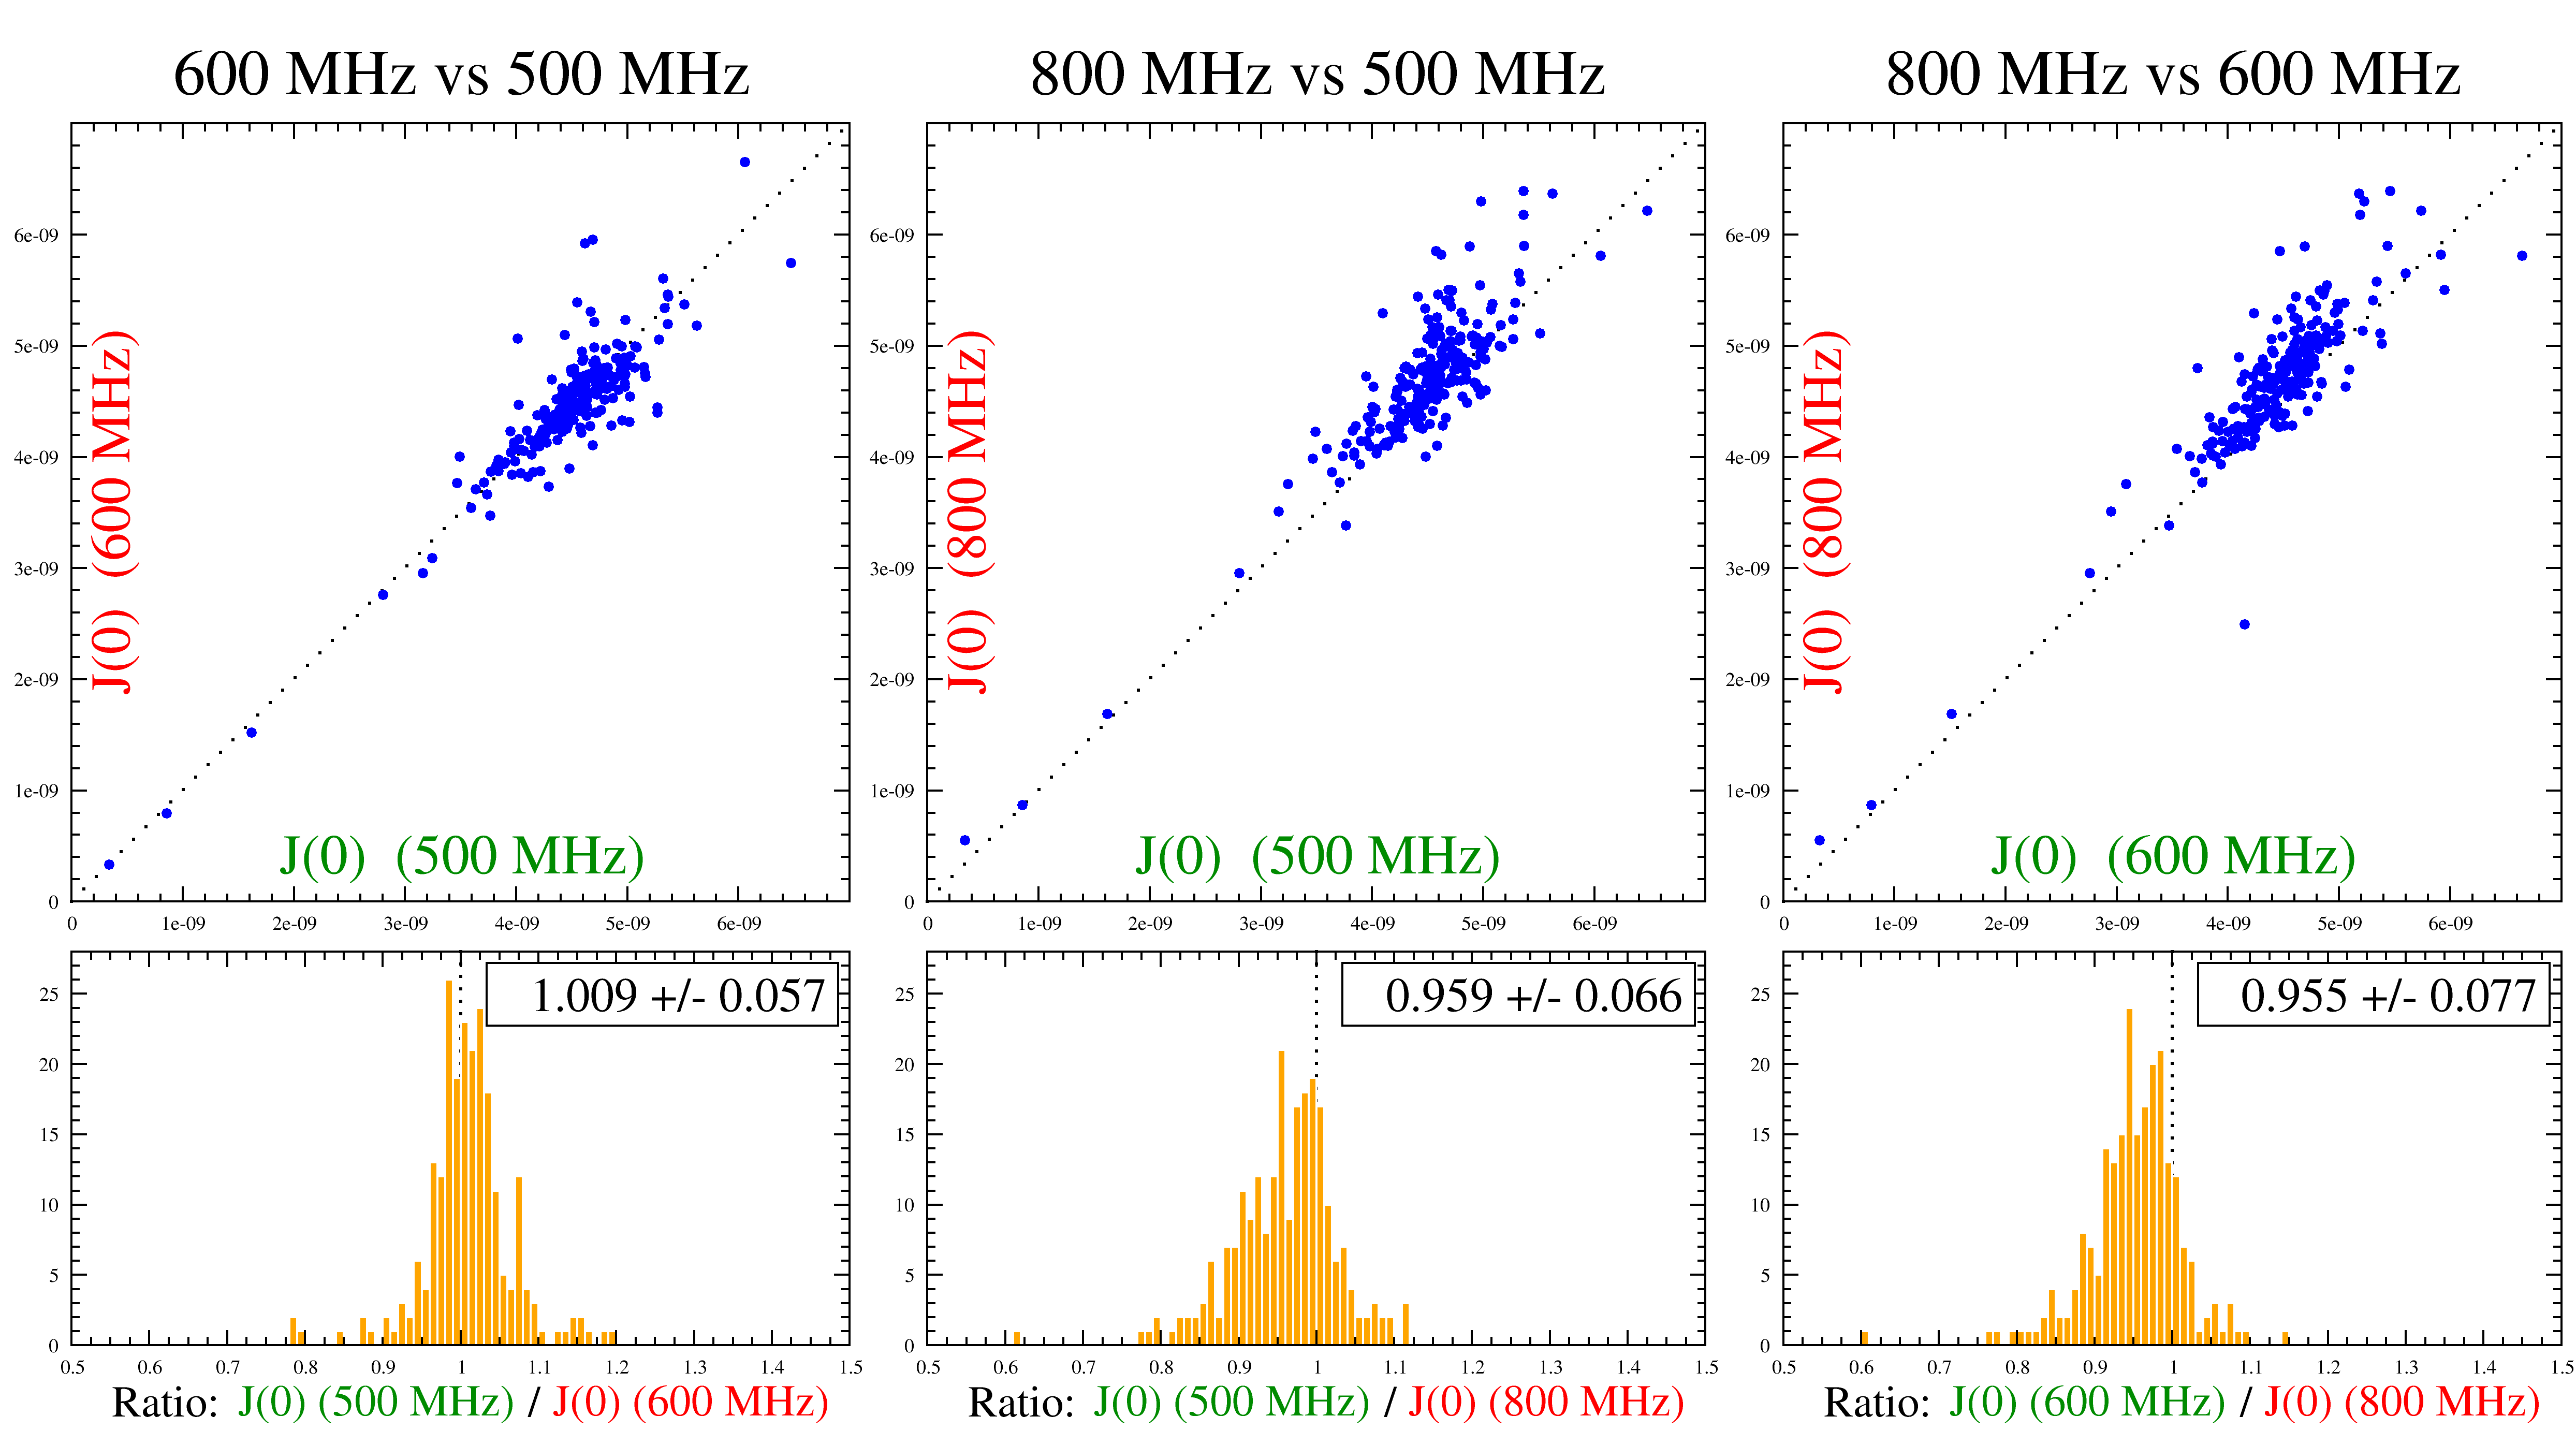
\includegraphics[
      width=0.9\textwidth,
      bb=5 2 1244 669
    ]
    {graphics/analyses/consistency_testing/consistency__J0_PSE-4}
  }
  \caption[Example of consistency testing visual analysis]{
    Example of consistency testing visual analysis.
    Relaxation data from three different magnetic fields are compared.
    For each pair of magnetic field, a correlation plot of the calculated $J(0)$ values (approach A, top) as well as an histogram of the ration of calculated $J(0)$ values (approach B, bottom) are shown.
    These graphs must be manually created from the output of the sample script shown in section~\ref{sect: consistency tests - sample script}.
    The PSE-4 data, as published in \citet{MorinGagne09b}, has been reused for the purpose of this example.
  }
  \label{fig: consistency analysis}
\end{figure*}

An example of such an analysis is shown in Figure~\ref{fig: consistency analysis}.
This example displays both consistent and inconsistent data.
As the figure shows, the data recorded at 500 MHz and 600 MHz are consistent with each other whereas the data recorded at 800 MHz is consistent with the neither the 500 MHz nor 600 MHz data.
Since more than two magnetic fields were used, this allowed the identification of the 800 MHz data as being inconsistent allowing the authors to take special care with this data set.

The 800 MHz data inconsistency is seen in the correlation plots (top) by a deviation from the dotted line (which represents the theoretical situation when equal $J(0)$ values are extracted from both magnetic fields.
It is also observable in the histograms (bottom) where the ratio of the data from two magnetic fields is not centered at 1.0.
In fact, there seems to be a systematic shift of the calculated $J(0)$ values at 800 MHz when compared to the two other magnetic fields.
This is caused by a similar shift in the experimental $\Rtwo$ (transversal relaxation rate) data.

For the 500 MHz and 600 MHz data pair, the data are centered around the dotted line in the correlation plot (approach A, top left) as well as centered around a value of 1.0 in the histogram comparing the ratios of values from both magnetic fields (approach B, bottom left).
Of course, there are some outlier values even in the case of consistent data.
There are caused by specific dynamic characteristics of these spins and are different from systematic inconsistencies such as depicted in the example above with the data recorded at 800 MHz.
